\section{Trigger and Data Acquisition Systems}
\label{sec:daq}

The signals from each detector's PMTs (or in the case of the drift chambers,
each wire) are digitized by ADC250~\cite{fADC_manual} flash analog-to-digital
converters (fADCS) or CAEN V1190~\cite{CAEN_1190_manual} time-to-digital
converters (TDCs).
% TODO: describe fADC mode 9 output (pulse pedestal, amplitude, integral, time)

The HMS detector hut contains a VXS crate with TDCs that process signals from
the HMS drift chambers.
The SHMS detector hut contains a VXS crate with fADCS that process signals from
the SHMS calorimeter's preshower and shower PMTs, and a VME crate with TDCs
that process signals from the SHMS drift chambers.
The Counting Room contains TDCs and fADCs to process signals from all the other
detectors, as well as sums of signals from other detectors.
These sums form ``pretrigger'' signals that are sent to a Trigger Interface
(TI) module which then distributes a specified trigger signal to synchronize
readout of the fADCs and TDCs in every read-out controller (ROC).
This analog trigger signal is called a ``Level 1 Accept,'' or L1 for short.
A copy of the Level 1 pretrigger is sent to every ROC which, when subtracted
from the raw TDC time, improves timing resolution from $\sim$\SI{25}{ns} to
$\sim$\SI{0.1}{ns}.
Both spectrometers have a TI, allowing them to be run independently or in
coincidence.


A broad overview of the SHMS trigger and readout system is given
in~\ref{fig:trigger_block_diagram}.
The HMS system is similar in structure, the largest differences being in in the
calorimeter signal chain.

% TODO: fix Cherenkov in diagram. The split signal goes to the fADC and analog
% sum. The sum goes to the fADC and to a discriminator. The bottom
% discriminator leg shouldn't be there.
\begin{figure}[!h]
    \centering
    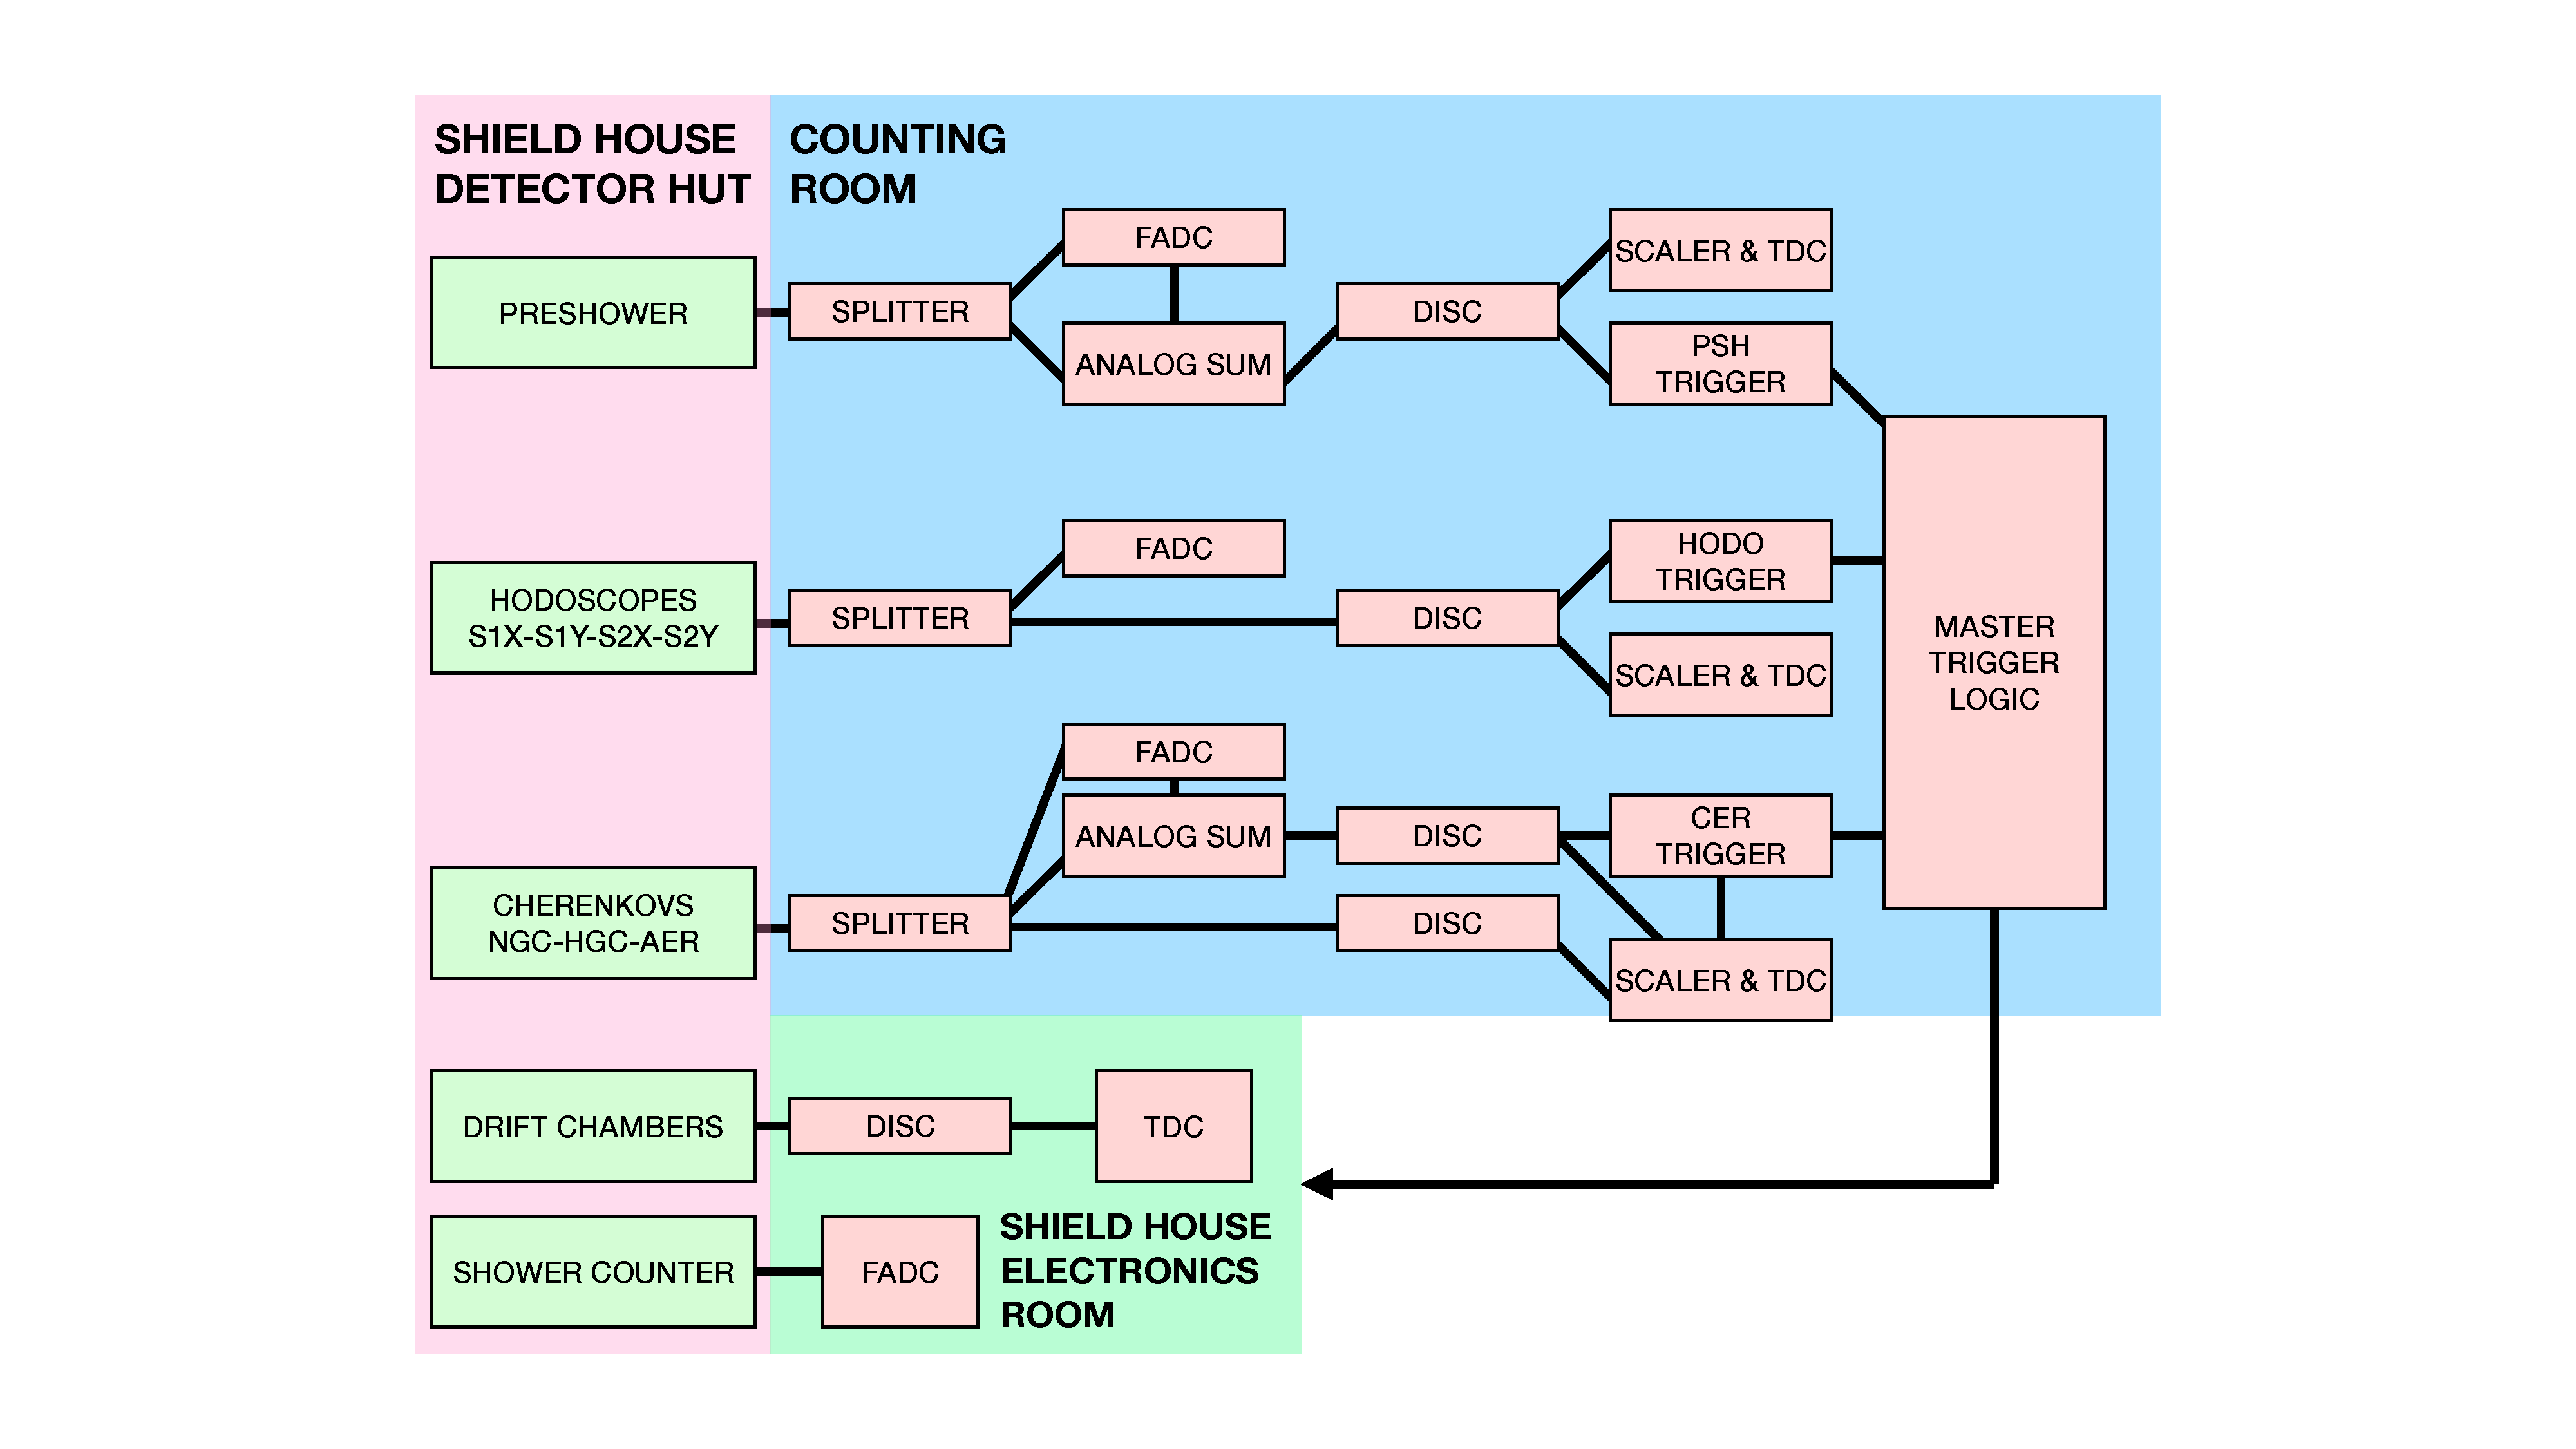
\includegraphics[width=0.9\textwidth]{chap3/trigger_block_diagram.pdf}
    \caption{Schematic diagram of the trigger system.
             Adapted from H. Fenker and B. Sawatzky.
             }
    \label{fig:trigger_block_diagram}
\end{figure}

Every trigger and pretrigger described below is sent to TDCs to keep track of
timing information necessary for event reconstruction, and scalers that count
every trigger with negligible deadtime.

\subsection{Pretriggers, TDC, and fADC Logic}
\subsubsection{Hodoscope}
Each hodoscope consists of 4 planes of scintillator paddles, with a PMT mounted
on both sides of each paddle.
The signal from each PMT is sent to a passive splitter.
One third of the signal amplitude is sent to an fADC, and the other two thirds
are sent to a discriminator.
The discriminator outputs are sent to daisy-chained TDCs and scalers, as well
as a LeCroy 4564 logic unit.
The logic unit computes a per-plane pretrigger by taking the AND of both sides'
$N$-fold ORs of each side's $N$ PMTs.
For instance, let h1X+ denote the 16-fold OR of the 16 PMTs on the left side of
the 1X plane of the HMS hodoscope and similarly h1X- denote the equivalent OR
of the right hand side.
Then the h1X plane pretrigger is the AND of h1X+ and h1X-.
The equations below describe the logic of each plane of the HMS and SHMS
hodoscopes' pretriggers\footnote{Because the SHMS 2Y plane has more PMTs than
each logic unit has channels, each side's 21-fold OR is actually an OR of a
16-fold OR and a 5-fold OR.}.
\begin{align*}
    \text{h1X = h1X+ (16-fold OR) AND h1X- (16-fold OR)} \\
    \text{h1Y = h1Y+ (10-fold OR) AND h1Y- (10-fold OR)} \\
    \text{h2X = h2X+ (16-fold OR) AND h2X- (16-fold OR)} \\
    \text{h2Y = h2Y+ (10-fold OR) AND h2Y- (10-fold OR)}
\end{align*}
\begin{align*}
    \text{p1X = p1X+ (13-fold OR) AND p1X- (13-fold OR)} \\
    \text{p1Y = p1Y+ (13-fold OR) AND p1Y- (13-fold OR)} \\
    \text{p2X = p2X+ (14-fold OR) AND p2X- (14-fold OR)} \\
    \text{p2Y = p2Y+ (21-fold OR) AND p2Y- (21-fold OR)}
\end{align*}

These pretriggers are converted from ECL twisted-pair to NIM signals by sets of
P/S model 7126 16-channel logic level translators~\cite{PS7126_manual}.
The NIM pretrigger signals are converted to variable-width gates by sets of P/S
model 752 logic units~\cite{PS752_manual}.
Sets of P/S Model 755 logic units~\cite{PS755_manual} generate the following
pretriggers for both spectrometers based on concidences of hodoscope plane
pretriggers:

\begin{itemize}
    \item S1 = 1X OR 1Y
    \item S2 = 2X OR 2Y
    \item STOF = S1 AND S2
    \item HODO 3/4 = coincidence of at least 3 planes
\end{itemize}

\subsubsection{Calorimeters}
Both spectrometer's calorimeters consist of two (SHMS) to four (HMS) layers of
long lead-glass blocks connected to PMTs on one or both sides.


The signals from the HMS calorimeter PMTs are read out in the Counting Room,
where they pass through a passive 50:50 splitter, with one half of each signal
sent to fADC inputs.
The other half is sent to P/S model 740 analog sum modules~\cite{PS740_manual}
which generate sums for each side of each layer (hA+, hA-, hB+, hB-, hC, and
hD\footnote{The third and fourth layers of the HMS calorimeter only have PMTs
connected to one side.}).
A LeCroy model 428F~\cite{LeCroy428F_manual} module sums both sides of the
first two layers to form hA and hB.
Each layer's sum is then sent to an fADC as well as a P/S model 715
discriminator~\cite{PS715_manual} to form the following calorimeter
pretriggers:

\begin{itemize}
    \item hPreSH LO = hA < \SI{-40}{mV}
    \item hPreSH HI = hA < \SI{-60}{mV}
    \item hShower LO = hA + hB + hC + hD < \SI{-45}{mV}
\end{itemize}


The SHMS calorimeter shower counter PMTs are all sent directly to fADCs inside
the electronics hut.
As in the HMS, each SHMS preshower layer PMT's output passes through a passive
50:50 splitter, with half the signal amplitude sent to an fADC and the other
half sent to analog sum modules that generate preshower LO/HI pretriggers.

\subsubsection{Cherenkovs}
All the threshold Cherenkov detectors in both spectrometers consist of some
medium in (some types of) charged particles generate Cherenkov radiation in the
visible spectrum and some number of PMTs that collect this light.
The output of each PMT is read out in the Counting Room, where it passes
through a passive 50:50 splitter.
One half of the signal amplitude is sent to an fADC, and the other half is sent
to a LeCroy 428F summing module~\cite{LeCroy428F_manual}.
This sum is sent to an fADC as well as to a P/S model 715
discriminator~\cite{PS715_manual} to form a pretrigger for that Cherenkov

\subsubsection{Other Pretriggers}
Four other pretrigger signals are generated from combinations of pretrigger
signals described above.
They are as follows:

\begin{itemize}
    \item EL-Hi = (HODO 3/4) AND (PreSH HI)
    \item EL-Lo = (Two of three from {HODO 3/4, STOF, PreSH LO}) AND (Cer)
    \item EL-Real = EL-Hi OR EL-Lo
    \item EL-Clean = EL-Hi AND EL-Lo
\end{itemize}

\subsubsection{Electronic Dead Time Measurement (EDTM) Pulser}
\label{sec:edtm}
To estimate the deadtime due to all electronics involved in data acquisition, a
pulser with a low frequency (\SI{3}{\hertz} in our experiment) is inserted into the
trigger logic.
The EDTM pulser fires every trigger in the system, and is also sent to its own
TDC and scaler channels.
By comparing the number of accepted EDTM triggers to the number of EDTM trigger
counts seen by the scaler, one can estimate deadtime.
This process is discussed in more detail in Section~\ref{sec:livetime}.

\subsection{Reference Times}
The reference time for an event is an OR-ed version of pretrigger signals
distributed to each fADC and TDC in every ROC.
The TDC modules have two internal clocks, one with a \SI{40}{MHz} cycle and one
with a \SI{10}{GHz} cycle.
When a given detector signal is received by a TDC, the digitized time latches
onto the leading edge of the 40 MHz cycle, yielding a timing resolution of
$\sim$\SI{25}{ns}.
We feed a \textit{reference time}, a copy of the pretrigger (common to all
fADCs and TDCs in a given ROC), to the TDC which will latch onto the leading
edge of the faster \SI{10}{GHz} clock.
The \textit{hcana} analyzer subtracts the reference time from detectors' raw
TDC times to yield a timing resolution of $\sim$\SI{0.1}{ns}.
This process is discussed in more detail in Section~\ref{sec:reftime}.
